%----------------------------------------------------------------------------------------
%	PACKAGES AND OTHER DOCUMENT CONFIGURATIONS
%----------------------------------------------------------------------------------------

\documentclass[final,hyperref={pdfpagelabels=false},20pt]{beamer}

% \documentclass[20pt]{beamer}

\usepackage[size=custom,width=76.2,height=106.68,scale=1.2,orientation=portrait]{beamerposter}
% Use the beamerposter package for laying out the poster with a portrait orientation and 30'' by 42'' paper size

\usetheme{I6pd2} 
% Use the I6pd2 theme supplied with this template

\usepackage[english]{babel} 
% English language/hyphenation

\usepackage{amsmath,amsthm,amssymb,latexsym} 
% For including math equations, theorems, symbols, etc

%\usepackage{times}\usefonttheme{professionalfonts}  % Uncomment to use Times as the main font
%\usefonttheme[onlymath]{serif} % Uncomment to use a Serif font within math environments

\boldmath 
% Use bold for everything within the math environment

\usepackage{booktabs} 
% Top and bottom rules for tables

\usepackage{natbib}
% added for bibtex

\graphicspath{{figures/}} 
% Location of the graphics files

\usecaptiontemplate{\small\structure{\insertcaptionname~\insertcaptionnumber: }\insertcaption} 
% A fix for figure numbering

%----------------------------------------------------------------------------------------
%	TITLE SECTION 
%----------------------------------------------------------------------------------------

\title{\huge Hierarchical Storage for Building Management System}
% Title

\author[AuthorNames]{Zhehao Wang\inst{1}, Jiayi Meng\inst{2}, Jeff Burke\inst{3}}
\institute[Institutes]{\inst{1} \inst{2} \inst{3} UCLA REMAP}

%----------------------------------------------------------------------------------------
%	FOOTER TEXT
%----------------------------------------------------------------------------------------

\newcommand{\leftfoot}{NDNComm, Sept 28th, 2015} % Left footer text
\newcommand{\rightfoot}{zhehao@remap.ucla.edu} % Right footer text

\begin{document}

\addtobeamertemplate{block end}{}{\vspace*{2ex}} % White space under blocks

\begin{frame}[t] % The whole poster is enclosed in one beamer frame

\begin{columns}[t] % The whole poster consists of two major columns, each of which can be subdivided further with another \begin{columns} block - the [t] argument aligns each column's content to the top

\begin{column}{.02\textwidth}\end{column} % Empty spacer column

\begin{column}{.465\textwidth} % The first column

%----------------------------------------------------------------------------------------
%	Introduction
%----------------------------------------------------------------------------------------

\begin{block}{Introduction}

Building management system (BMS) is a sensor data acquisition system which automatically manages a building's heating, ventilation and air conditioning, and other systems. \newline
An NDN based BMS leverages the architecture's advantages in hierarchical data naming and name-based routing and forwarding, in-network caching, and inherent security support, and may overcome the challenges IP faced, namely complexity of network addressing and configuration, reliance on middleware, and a lack of security \cite{wentao-bms}. \newline
This summer's work focuses on the data aggregation and signing/verification in NDN BMS, and updates the previous work by Wentao.

\end{block}

%----------------------------------------------------------------------------------------
%	Design Objectives
%----------------------------------------------------------------------------------------

\begin{block}{Design Objectives}

\begin{itemize}
\item{Hierarchical storage and aggregation}
\end{itemize}
Objective: Design a hierarchical storage approach and a stream-based approach to calculaIng aggregates, distribuIng processing and taking advantage of local storage.

% Quoted from summer opening slides by Wentao and Jeff

\begin{itemize}
\item{BMS data signing and verification}
\end{itemize}

\end{block}

%------------------------------------------------
%   Design overview
%------------------------------------------------

\begin{block}{Design Overview}

Figure \ref{fig:namespace} illustrates the namespace of the BMS application, and Figure \ref{fig:example-name} illustrates an example name of a piece of BMS data.

\begin{figure}
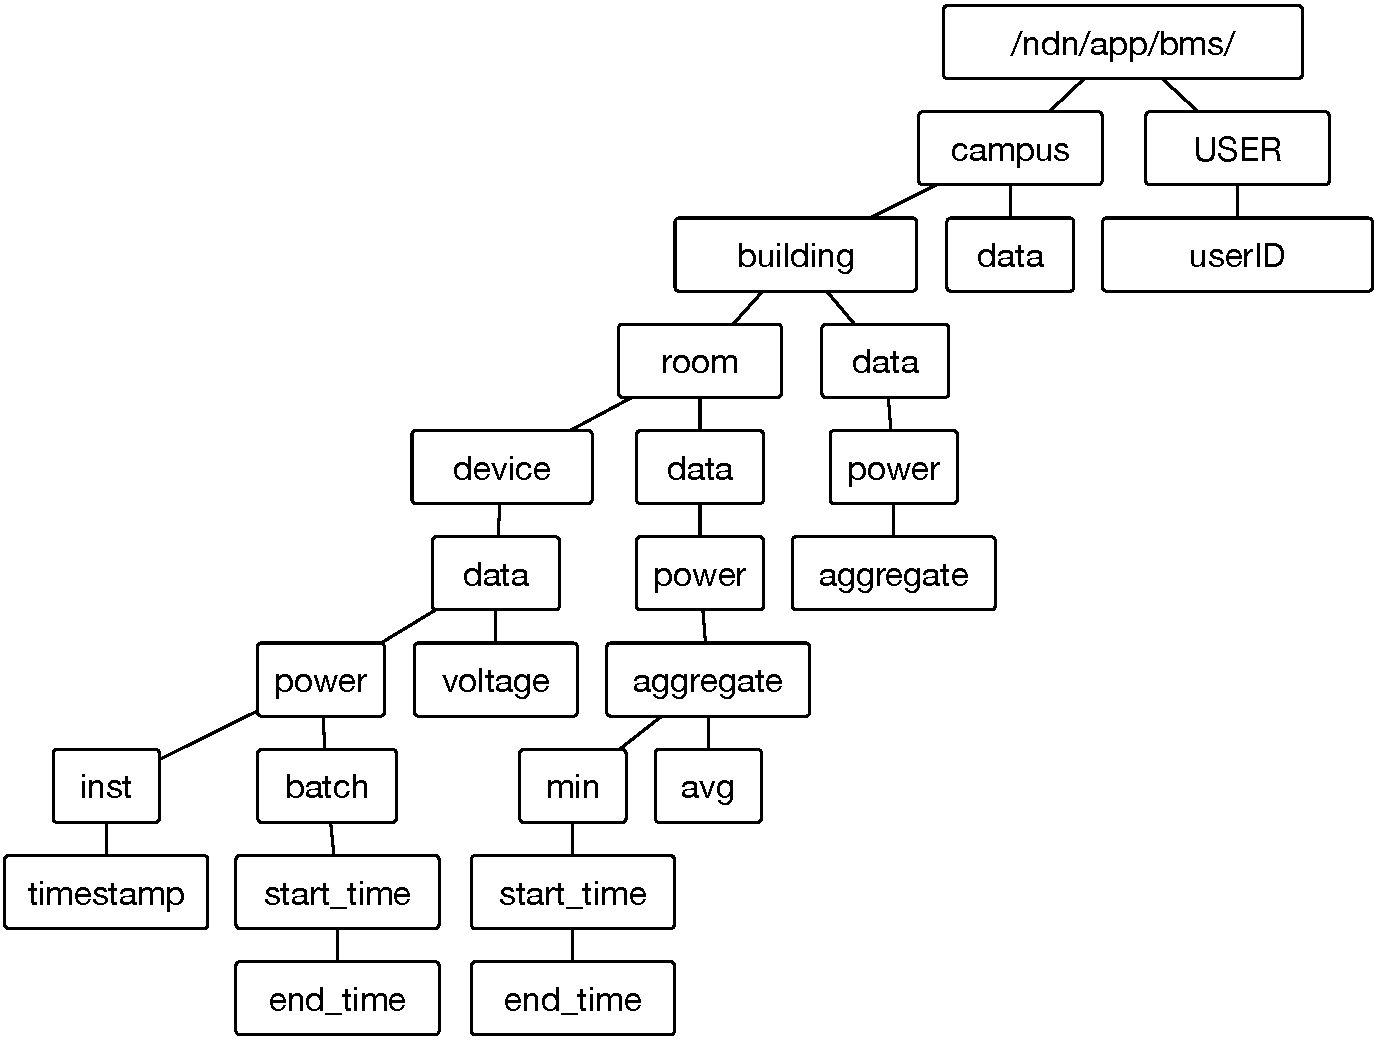
\includegraphics[width=0.8\linewidth]{bms-namespace-update-Sep19}
\caption{BMS namespace}
\label{fig:namespace}
\end{figure}


\begin{columns}[T]

\begin{column}{.45\textwidth}
\begin{itemize}
\item{Physical location branch represents the hierarchical structure of BMS data, organized in Campus - Building - Room - Device}
\item{User branch records the list of BMS user identities, to be used by GBE later}
\end{itemize}
\end{column}

\begin{column}{.50\textwidth}
\begin{figure}
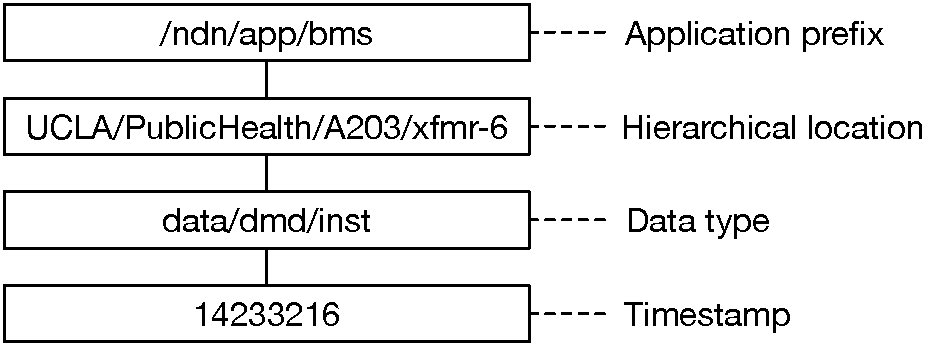
\includegraphics[width=0.9\linewidth]{bms-example-name}
\caption{Example BMS data name}
\label{fig:example-name}
\end{figure}
\end{column}

\end{columns}

\end{block}

%----------------------------------------------------------------------------------------
%	Data Aggregation
%----------------------------------------------------------------------------------------

\begin{block}{Data Aggregation}

\begin{columns}[T]

\begin{column}{.45\textwidth}
\begin{itemize}
\item{Leaf nodes publish aggregated data at fixed time window.}
\item{Non-leaf aggregate the data after all children respond, and publish data with the same time window.}
\item{Long lived interests for fixed time window moves data across layers.}
\end{itemize}
\end{column}

\begin{column}{.50\textwidth}
\begin{figure}
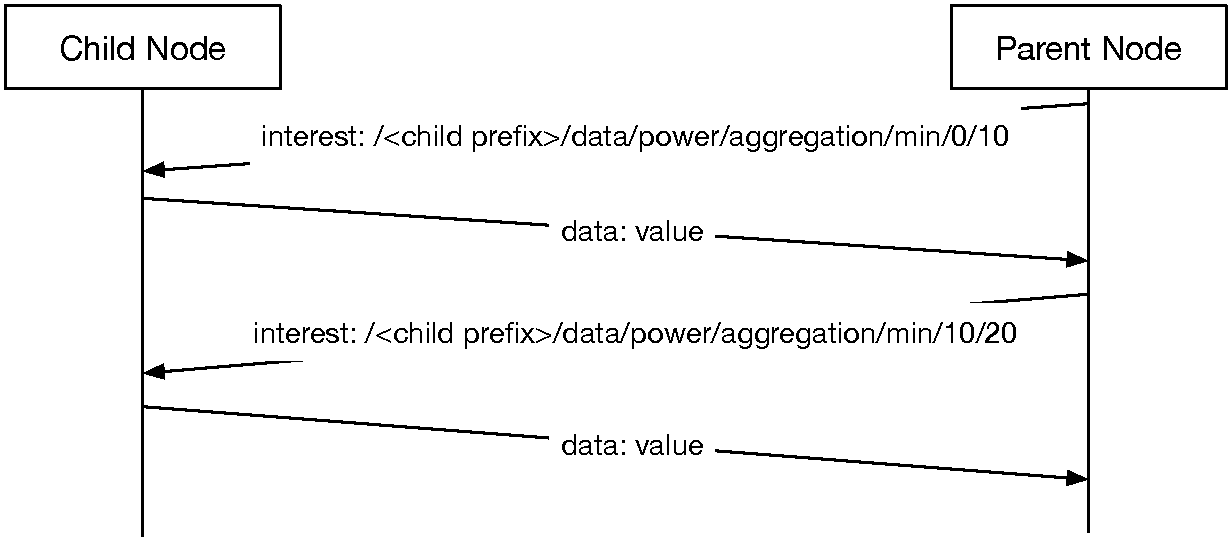
\includegraphics[width=\linewidth]{bms-move-aggregate-sequence}
\caption{BMS move aggregation sequence}
\label{fig:move-aggregation}
\end{figure}
\end{column}

\end{columns}

\end{block}

%-----------------------------------
\end{column} % End of the first column

\begin{column}{.02\textwidth}\end{column} % Empty spacer column
 
\begin{column}{.465\textwidth} % The second column

%----------------------------------------------------------------------------------------
%	Trust Schema
%----------------------------------------------------------------------------------------

\begin{block}{Trust Schema and Bootstrapping}

\begin{itemize}
\item{BMS data should be verified hierarchically}
\item{The certificates of BMS children node should be signed by their parent nodes in the tree}
\item{Campus certificate is the root of trust for BMS data and user. (not so in namespace)}
\end{itemize}

\begin{columns}[T]

\begin{column}{.25\textwidth}

\begin{figure}
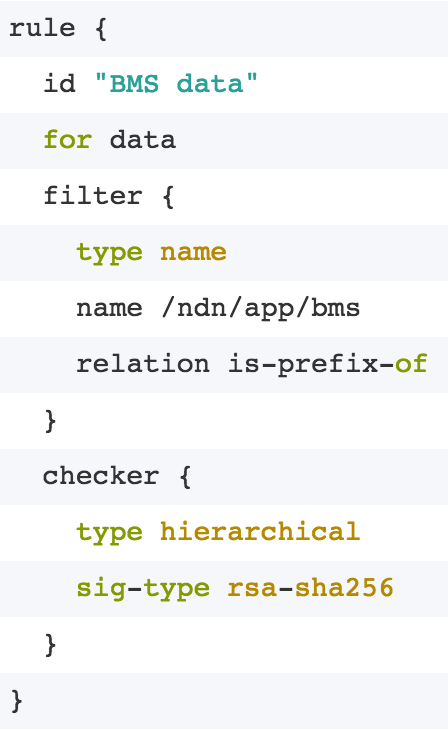
\includegraphics[width=\linewidth]{trust-schema-data.png}
\label{fig:trust-schema-data}
\end{figure}
\end{column}

\begin{column}{.63\textwidth}
\begin{figure}
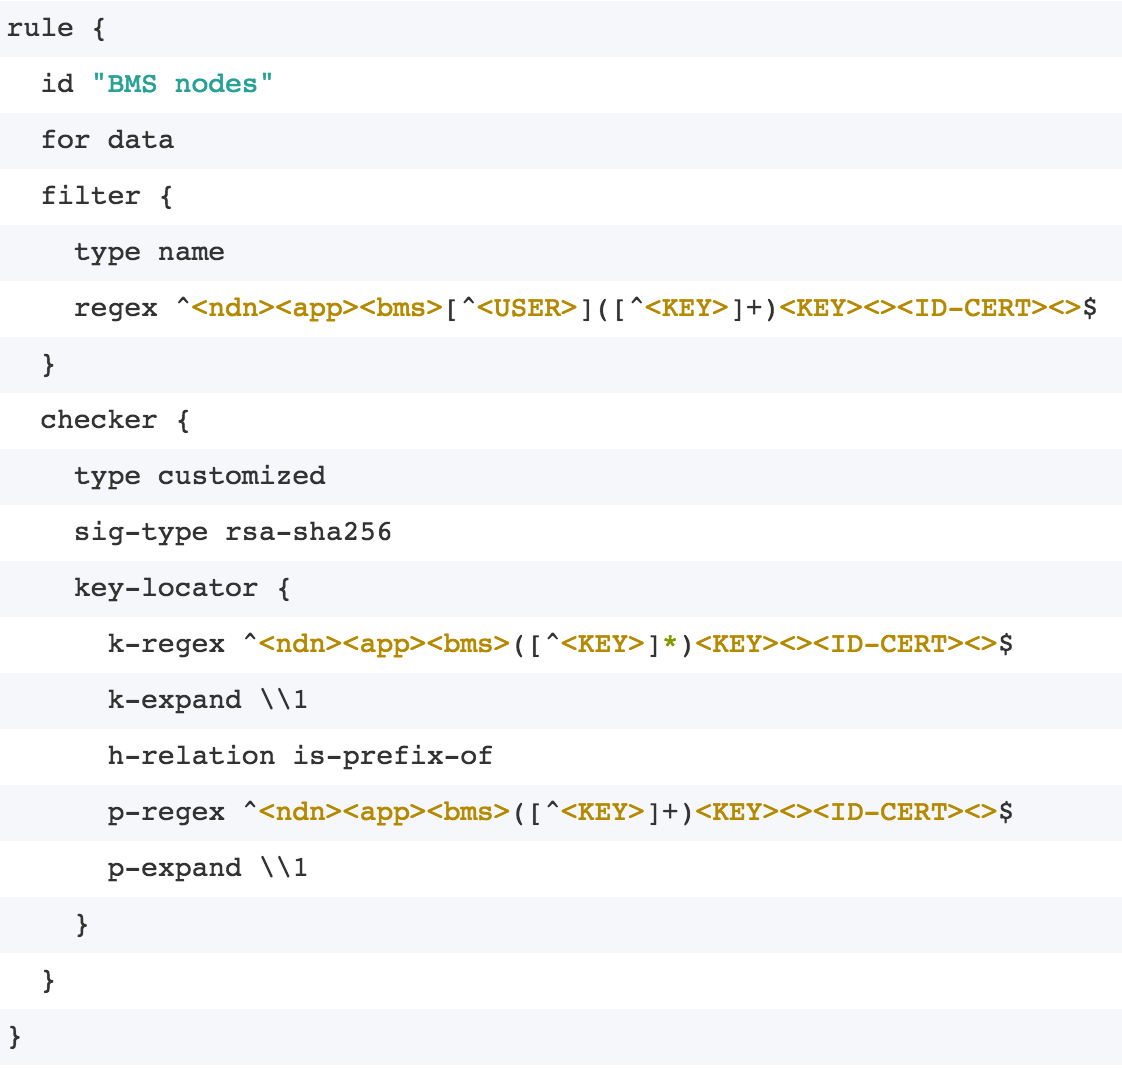
\includegraphics[width=\linewidth]{trust-schema-nodes.png}
\label{fig:trust-schema-nodes}
\end{figure}
\end{column}

\end{columns}

\vspace{18mm}

\begin{columns}[T]

\begin{column}{.26\textwidth}
\begin{itemize}
\item{Bootstrap:}
\end{itemize}
Each BMS children node should obtain a valid certificate from the parent when joining the network for the first time. Figure \ref{fig:add-child-sequence} illustrates this process.
\end{column}

\begin{column}{.66\textwidth}
\begin{figure}
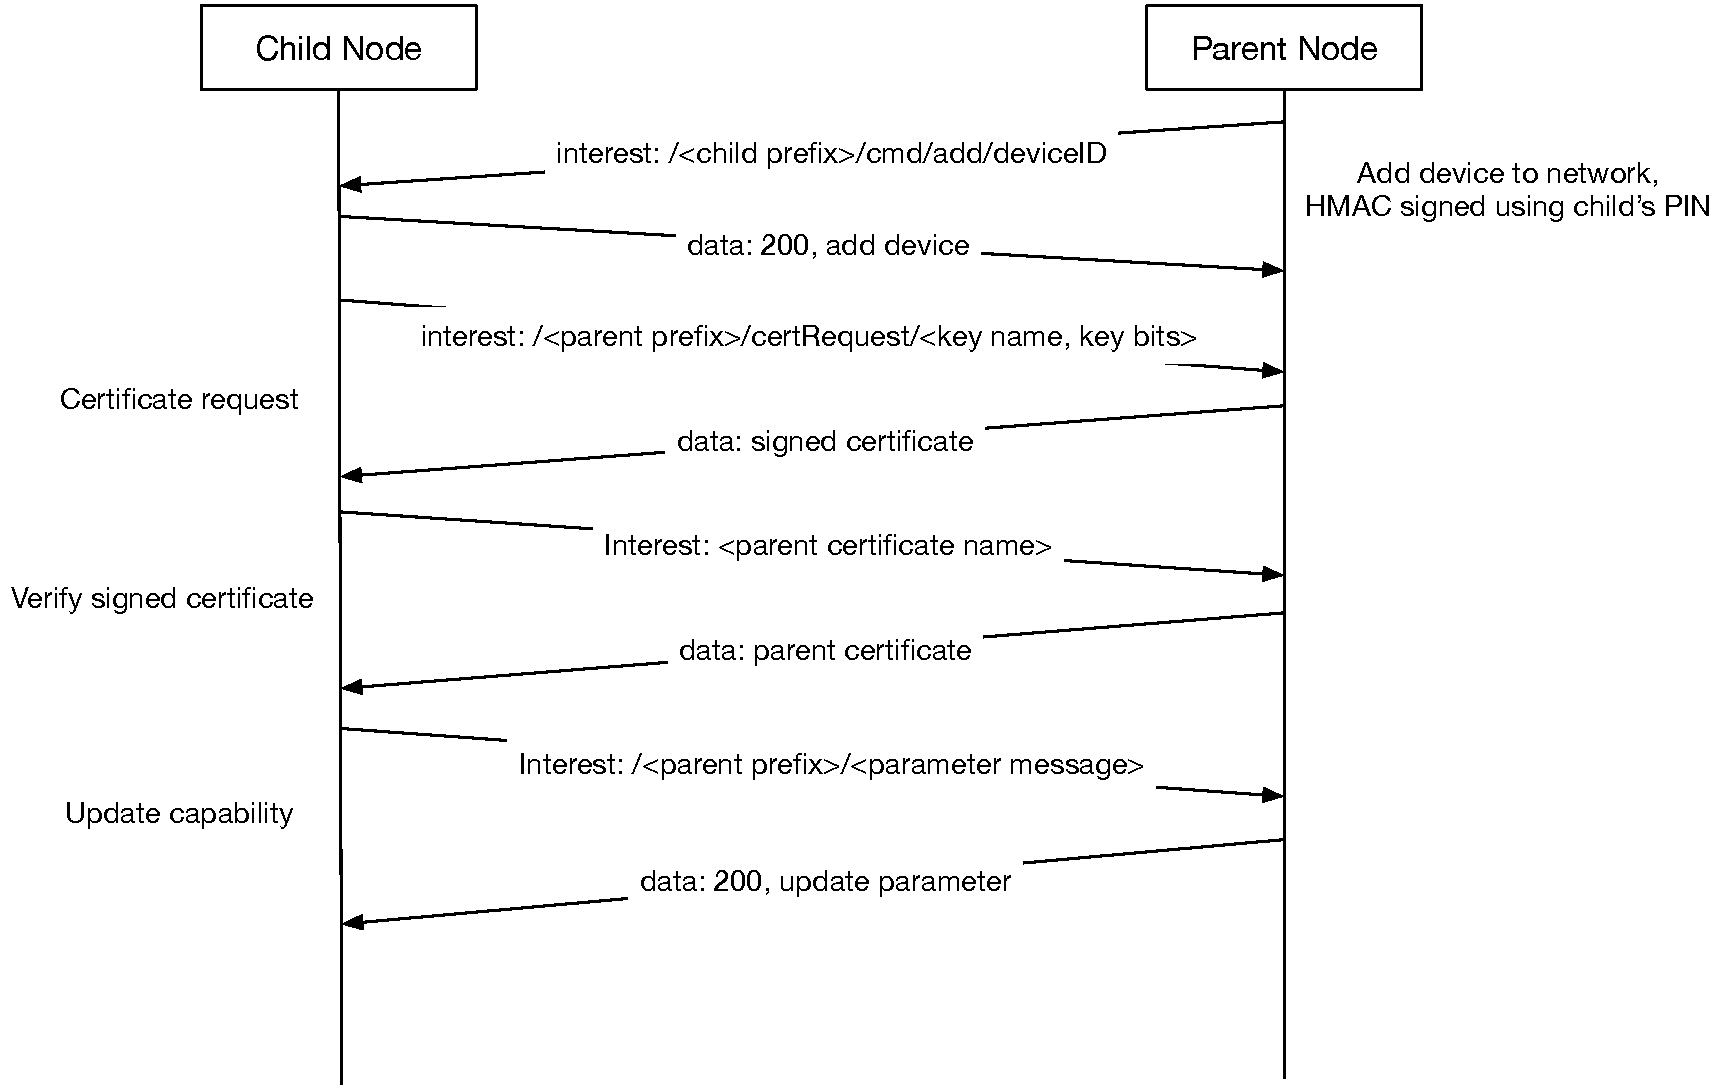
\includegraphics[width=\linewidth]{bms-add-child-sequence}
\caption{BMS add child sequence}
\label{fig:add-child-sequence}
\end{figure}
\end{column}

\end{columns}

\end{block}

%----------------------------------------------------------------------------------------
%	Demo Implementation
%----------------------------------------------------------------------------------------

\begin{block}{Demo Implementation}

As illustrated in Figure \ref{fig:node-structure}, we are running BMS aggregation nodes in mini-ndn, with connection to the NDN testbed and BMS data publisher gateway node. \newline
An in-browser visualization interface, as demonstrated in Figure \ref{fig:bms-ui} is being developed.

\begin{columns}[T]

\begin{column}{.44\textwidth}
\begin{figure}
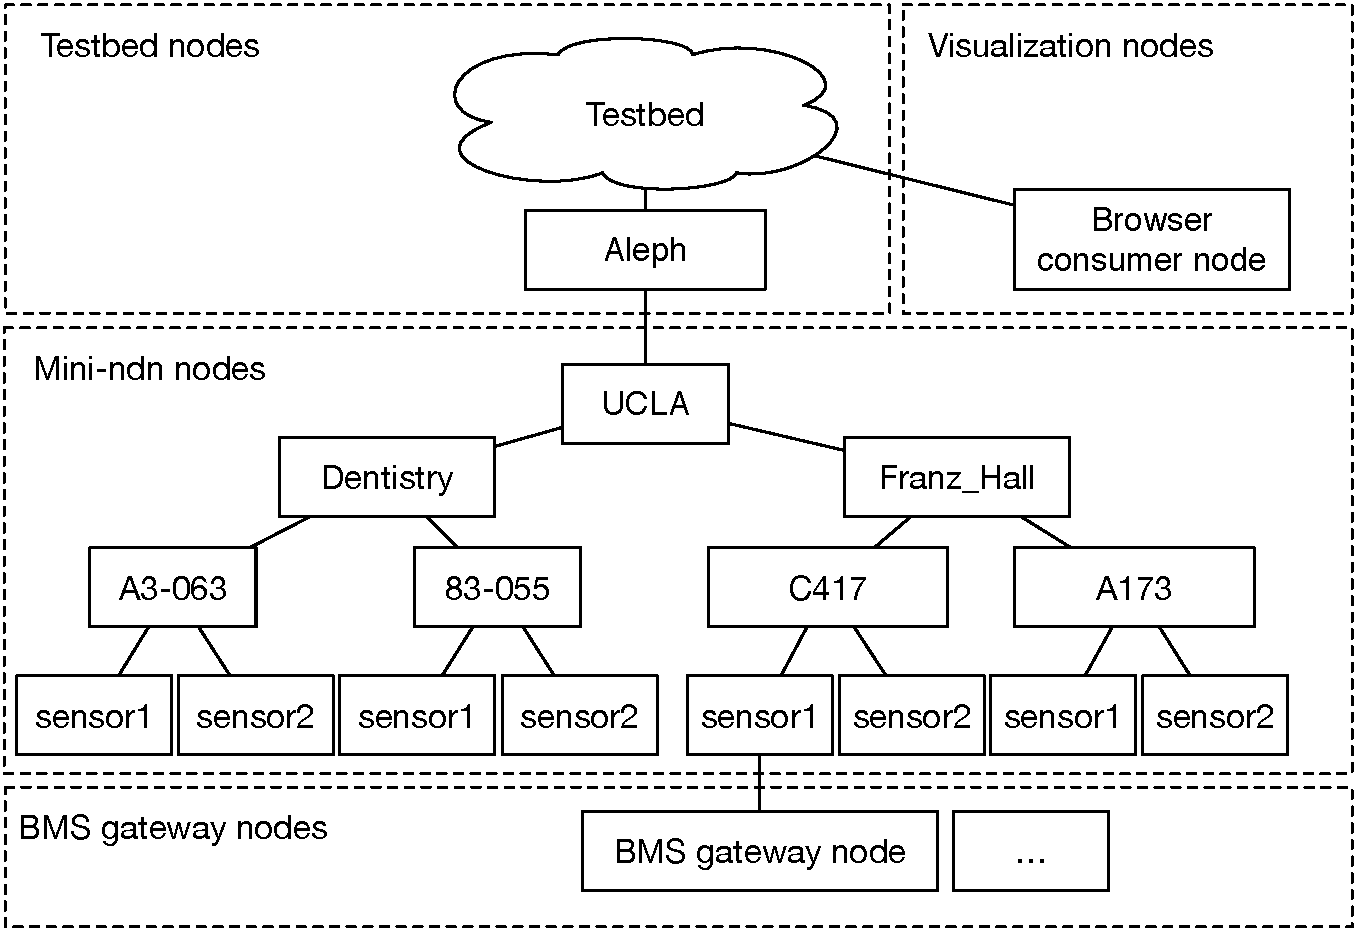
\includegraphics[width=1\linewidth]{bms-nodes-structure}
\caption{BMS deployment structure}
\label{fig:node-structure}
\end{figure}
\end{column}

\begin{column}{.48\textwidth}
\begin{figure}
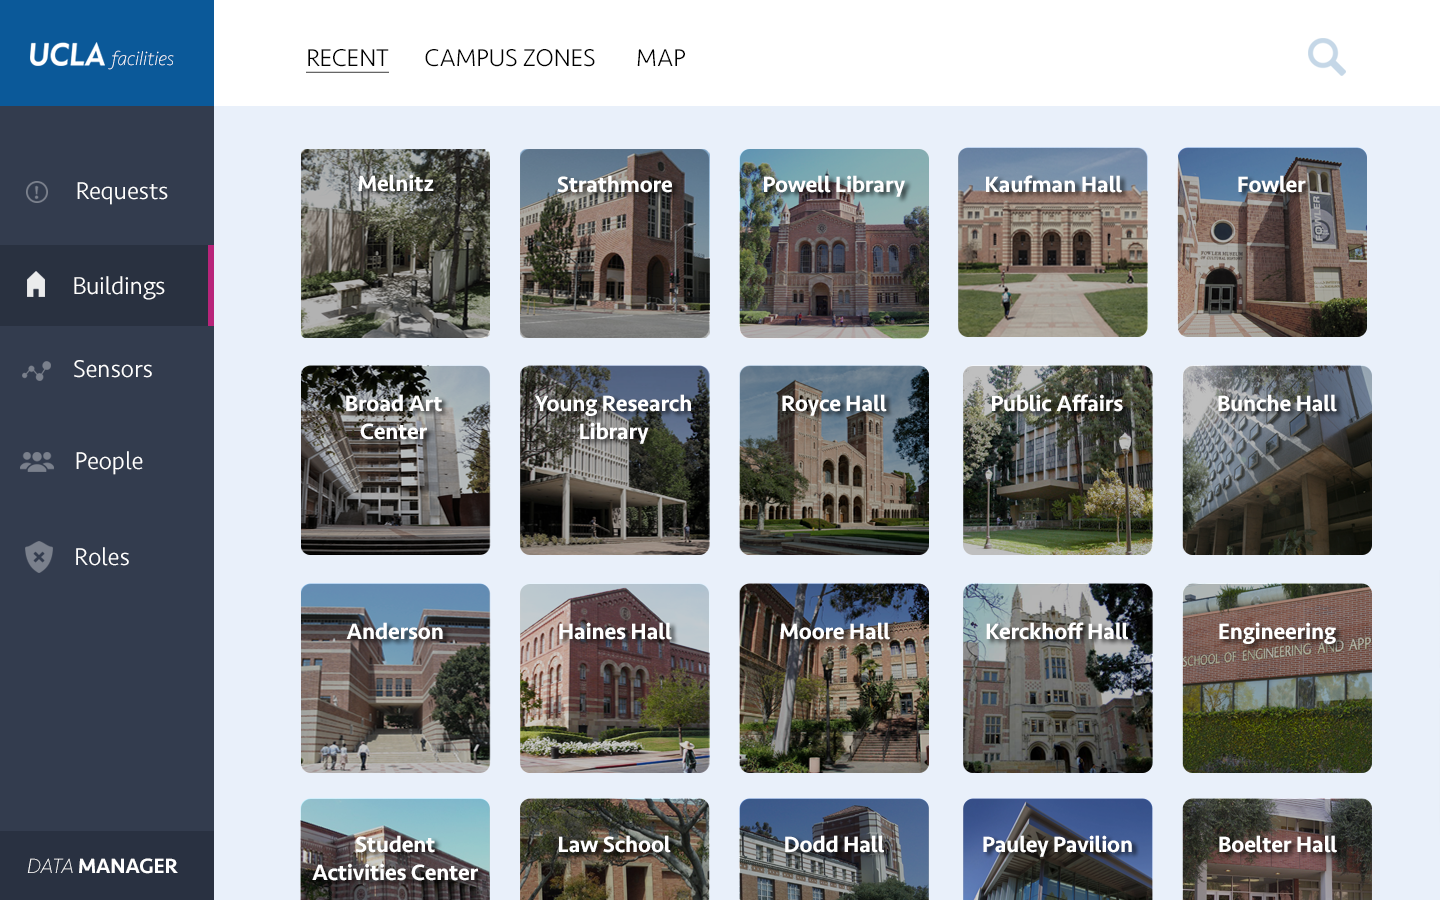
\includegraphics[width=\linewidth]{bms-ui-demo.png}
\caption{BMS UI demo}
\label{fig:bms-ui}
\end{figure}
\end{column}

\end{columns}

\end{block}

%----------------------------------------------------------------------------------------
%	Conclusion & Future Work
%----------------------------------------------------------------------------------------

\begin{block}{Future Work}
\begin{itemize}
\item Access control / GBE in BMS
\item In-browser consumer interface
\item Namespace update? Mentioned earlier about some unresolved issues?
\end{itemize}
\end{block}

%----------------------------------------------------------------------------------------
%	REFERENCES
%----------------------------------------------------------------------------------------

\begin{block}{References}
        
\nocite{*}
% Insert publications even if they are not cited in the poster
\small{\bibliographystyle{unsrt}
\bibliography{reference}}

\end{block}

%----------------------------------------------------------------------------------------
%	CONTACT INFORMATION
%----------------------------------------------------------------------------------------

\setbeamercolor{block title}{fg=black,bg=orange!70} % Change the block title color

\begin{block}{Contact Information}

\begin{itemize}
\item Email: \href{mailto:zhehao@remap.ucla.edu}{zhehao@remap.ucla.edu}
\end{itemize}

\end{block}

%----------------------------------------------------------------------------------------

\end{column} % End of the second column

\begin{column}{.015\textwidth}\end{column} % Empty spacer column

\end{columns} % End of all the columns in the poster

\end{frame} % End of the enclosing frame

\end{document}